%De l'importance et de la place de la communication externe dans l'associatif
%TODO remplacer le titre par celui de la fiche contrat pédagogique.

\section {Introduction}

    Depuis bientôt 4 ans, je suis mes études à l'Insa.
    La première chose que l'on m'a dite sur cette école, avant même son nom, concernait  l'importance de la composante humaine de la formation par rapport à d'autres établissements. Ce travail en est d'ailleurs la preuve.

    Depuis bientôt 4 ans, j'ai eu l'occasion de travailler dans plusieurs associations : le Ski Club, l'AEDI, le BDE, les 24h,  pour ne citer que les plus importantes.
    Toutes ces expériences ont en commun ma passion pour les arts graphiques et la communication visuelle.

        
    
\section{But de la communication extérieure}

    Le but premier de la communication est de promouvoir les services, ou actions d'une association.  (ou bien : de ces associations)
    Dans le cas du ski club, il s'agira des sorties proposées et de la location. Pour les 24h, ce sera la festival, et autres soirées ; pour le BDE, les services et évènements organisés.
    Mais on peut prendre aussi l'exemple du forum Rhône Alpe, de la plupart des associations de département etc ...

    Tout le travail effectué en communication extérieure est principalement tourné vers la promotion des autres actions faites par l'association.
    Un seul contre-exemple me vient à l'esprit : les cartes de vœux envoyées par les 24h à ses partenaires.  Mais, en un sens, il est encore question de promotion, puisque cela contribue à garder de bonnes relations ainsi qu'à pérenniser les partenariats commerciaux.


\section{Mes expériences dans l'associatif}

    \subsection{Le ski club}
        
        Depuis que je suis enfant,  j'ai la chance de skier chaque hiver. Pour poursuivre cette activité durant mes études, je me suis inscrit dès ma première année comme membre actif du Ski club.
        
        L'ancien webmaster quittait l'Insa l'année de mon arrivée, je me suis donc proposé de reprendre le site de l'association pour le maintenir.
        Ce fut ma première expérience relative à la communication dans l'associatif.
        J'ai entièrement reconstruit le site web, pour améliorer la visibilité en ligne de l'association.
        
        Le site comportait des informations concernant l'organisation des sorties, du weekend à venir, ainsi que sur la location ou l'entretien de matériel.
        
        Je ne fais plus parti du ski-club, le site a donc été remplacé par les membres actifs. (?!? qu'est-ce que tu veux dire ? Nouveau Webmaster au sein des membres actifs ? site remplacé par de la communication plus directe style panneaux dans l'école ? Ou bien est-ce que le site a depuis ton départ été modifié par les nouveaux adhérents de l'assoc' ?)
        
    \subsection{L'AEDI}
        
        Il serait faux de dire que je suis membre de l'AEDI. Je n'ai fait que proposer mon aider en cas de besoin.
        Mais j'ai eu l'occasion de dessiner un visuel de T-Shirt distribué aux "bizuth" lors du weekend d'intégration, et différentes affiches pour le barbecue de fin d'année.
        Ces travaux étaient d'une durée très courte, cela ne m'a pas empêché néanmoins d'en tirer de bonnes expériences. (lesquelles ? Cela donne envie de savoir ...)
        
    \subsection{Les 24 heures de l'Insa}
        
        Cela fait 2 ans que je suis dans l'équipe communication des 24h de l'INSA, et c'est probablement pour cette association que j'ai fourni le plus de travail.
        Durant ces deux années,  j'ai dessiné un certain nombre de ressources qui ont été réutilisées sur différents supports, tels que les programmes, les gobelets, les T-Shirts, les affiches etc ...
        J'ai également participé, entre autres, à l'élaboration des affiches journées et concerts.
        
        J'en tire de bonnes expériences notamment en ce qui concerne la suivi d'un projet sur une plus longue durée.(lesquelles : travail en équipe, accepter la remise en cause, avoir à travailler dans l'urgence, imaginer un dessin qui sera ensuite affiché en très grandes dimensions ?...)
        
    \subsection{Le BDE}
    
        J'ai également collaboré à plusieurs projets avec l'équipe communication du BDE.
        Cependant, ayant intégré l'équipe en cours d'année, je n'ai pas eu l'occasion de faire des travaux très significatifs.

\section{Observations}

    La première observation que j'ai pu faire aussi bien au sein de l'équipe com du BdE que des 24h, est que la communication externe n'est pas toujours à la hauteur pour promouvoir les efforts fournis par les autres services ; soit à cause d'un retard, d'un manque de moyens, ou d'un manque d'efficacité.

    \subsection{BdE}

        Par exemple, au BdE, comparativement (en comparaison à ...) à la médiatisation que l'on peut voir dans la plupart des entreprises, le BDE  a un service de communication sous-estimé et qui, je pense, devrait être plus important afin de mieux faire connaitre les services proposés aux étudiants. (pas très clair, à reformuler ou à développer. Rappelle-toi : lis à voix haute ce que tu écris pour vérifier si c'est bien compréhensible. Que veux-tu dire par "sous-estimé" ? peu connu, peu reconnu, peu efficace ?) Je suis conscient que ce n'est pas comparable à une entreprise commerciale, dont  la survie dépend en grande partie de sa visibilité. Malgré tout, %TODO Continuer
    
    \subsection{24 heures de l'Insa}
        
        En revanche, la communication aux 24h est plus importante et mieux planifiée, parce qu'indispensable à la manifestation, mais elle n'est souvent pas assez organisée pour avoir des ressources vraiment utilisables d'une année sur l'autre. (des fonds ? des revenus ? récupérables d'une année sur l'autre)
        Bien qu'un effort soit fait de ce côté là, et, pour donner un exemple, les photos prises sur la manifestation d'une année sur l'autre sont souvent réutilisées (mettre ici le "d'une année sur l'autre") dans plusieurs supports de communication, tels que le site web, ou les plaquettes destinées aux sponsors.
        
    Cependant, on peut nuancer cette remarque, en notant que d'une part, les services du BdE ne pâtissent pas de cette mauvaise visibilité, et sont toujours d'une grande aide aux étudiants. D'autre part, les 24h bénéficient déjà d'une grande notoriété auprès d'un certain public, et une campagne de communication faite au dernier moment ne nuit pas au festival, ni à son image. Le but est plus d'informer que d'attirer de nouveaux publics.
    %TODO remanier faites au dernier moment. (mise sur pieds in extremis ou montée/organisée en urgence ...)
    
\section{Déboires : pièges à éviter}

    Je vais revenir sur plusieurs gros projets, en analysant quels étaient les difficultés, les enjeux, et pourquoi ces projets n'ont pas abouti, ou mal aboutie (ou se sont mal déroulés ?).
    
    \subsection{La bache de la MdE}
    
        Le BdE ayant un partenariat important/conséquent avec Perstil, ceux-ci nous proposèrent une impression gratuite sur une bâche de 8m par 1m, avec pour seule contrainte, un bandeau publicitaire au bas de l'affiche. 
        La décision fut prise de placer cette bâche au devant de la MdE, sur la rambarde du balcon, pour attirer un peu plus l'œil et signaler la présence de la MdE.
        Quand je suis arrivé dans l'équipe, cette proposition était déjà lancés depuis quelques année, mais personne ne s'était mis à la tâche.
        Je me suis donc proposé de travailler dessus pendant l'été. Et après quelques réunions, le thème choisi serait "Urbano-floral".
        
        L'erreur que je peux relever ici, c'est qu'on entame un travail aussi important, 2 mots ne peuvent vraiment pas définir un thème. (J'ai très vite réalisé, face à une tâche et un travail aussi important, que le thème ne pouvait se résumer à deux mots. Il aurait été souhaitable de mieux définir le concept ciblé/recherché)
        
        Ainsi, je suis parti avec des idées en tête. Et chacun fit de même en interprétant le thème différemment.
        Pour la plupart des ébauches que je présentais, les membres de l'équipe étaient en désaccord, (Les membres de l'équipe étaient en désaccord avec la plupart des ébauches que je présentais, chacun ayant son idée en tête). Le projet finit par stagner, (un consensus ne pouvant se dégager) puisque plus rien n'était approuvé.
        
        Je pense donc qu'il aurait fallu, pour ce travail, ne pas s'arrêter à deux mots, mais réellement se mettre d'accord sur un style visuel, et sur les attentes du résultat.
        Pourquoi faire ce travail, qu'est ce qu'on attendra du résultat, dans quel registre peut-on se placer ? (C'est intéressant, tu peux développer un peu plus les idées que tu as eu à ce moment-là)
        %TODO à réécrire.
        
    \subsection{Les affiches Journées et Concerts des 24h}
        
        Un des travaux les plus important pour l'équipe communication des 24h est la réalisation des affiches Journées et Concerts.
        Ce sont deux affiches imprimées au format B1, en grand nombre et qui sont en grande partie responsables de la visibilité des 24h sur Villeurbanne et Lyon.
        
        Chaque année, des propositions de thèmes et des ébauches d'affiches sont présentées plusieurs mois avant la manifestation, afin que l'équipe entière des 24h puisse juger et voter pour un thème.
        L'an dernier, les deux idées qui s'étaient démarquées étaient une reprise des lapins suicidaires de Andy Riley, et un thème dont la ligne directrice était l'aspect BD.
        Nous avons alors choisi d'utiliser les 2 thèmes.
        %TODO inutile de détailler autant. (Si, les exemples rendent ton texte plus vivant et appuient tes idées) 
        J'avais une idée très précise de ce que je pensais faire, et elle semblait plaire à l'équipe.
        
        Entre-temps, l'idée des lapins suicidaires a été abandonnée, pour des raison évidentes.
        Nous avons donc remplacé dans la précipitation les lapins par des pandas, image plus positive.
        
        J'ai commencé à proposer des ébauches, et le travail avançait bien.
        Cependant, au fur et à mesure que j'avançais, de plus en plus de remarques m'ont été faites. Tel détail serait mieux ainsi, ou tel autre autrement, etc ...
        Au fur et à mesure que le travail avançait, le nombre de remarques augmentait, et plus j'approchais du résultat final, plus il semblait déplaire.
        C'est comme ça que, quelques jours avant l'envoi pour impression, il a été décidé de recommencer presque de zéro pour produire une affiche différente et exempte de toutes les remarques faites à la précédente.
        
        De mon avis, c'était un travail bâclé, bien plus critiquable que la précédente affiche, mais sous prétexte de la précipitation (par manque de temps, ou, pris par le temps) , l'avis général a été, "nous n'avons plus le temps de faire des remarques, il faut agir" -décision prise dans la précipitation. 
        
        Je pense que bien qu'il faut prendre en compte les remarques faites, il faut surtout prendre du recul, et éviter de les suivre automatiquement. (là, cela semble incohérent : faut-il prendre en compte les remarques ou éviter de les suivre ? à reformuler plus clairement) . Sinon, cela amène à perdre la cohésion de son idée, et le travail final perd de son intégrité.
        
        Pour exemple, je me suis penché sur la façon de procéder du festival Rock'n'Solex, qui est très proche des 24h de l'Insa (festival étudiant organisé par l'Insa de Renne).
        Ils ne travaillent pas eux-même sur l'affiche, mais lancent un concours (quid du thème ? 2 mots ou un concept plus développé ? car cela semble avoir été votre pb avec urbano-floral) . Ils ont une réputation suffisante pour que les travaux proposés soient d'une certaine qualité. (bonne qualité ou qualité certaine)
        Quelques modifications sont faites sur l'affiche gagnante, puis c'est l'impression.
        
        La grande différence, c'est qu'ils choisissent parmi des travaux déjà aboutis, complets, qui ont déjà un certain caractère et une intégrité.
        
        Je pense donc qu'il faut réduire le nombre de personne qui peuvent donner leur avis sur les travaux, afin de ne pas se perdre en modifications.
        Et seulement qu'une fois que le projet d'affiche est  abouti, le soumettre au reste de l'équipe. Dans tout les cas, ça ne pourra pas plaire à tout le monde. Mais un travail abouti est plus facilement acceptable qu'un travail sans cesse remanié, tout simplement parce que ceux qui travaillent dessus voient déjà la continuité, et l'aboutissement du projet de design sur lequel ils ont travaillé, alors que les autres non.
        %TODO à réécrire.
        
\section{Résultats et conclusion tiré de ces expériences}

    %TODO découper en sous parties

    De manière générale, dans l'associatif le travail fourni est important. Je pourrais estimer à 10\% le ratio de travaux qui seront effectivement publiés.

    Il y a effectivement une part du travail qui est dédiee à des essais, ou soumis à des sélections ; et également une part du travail qui ne sera jamais aboutie, ou abandonnée en cours de route.

    La principale cause de ce gaspillage est la méthode employée : en effet, il est plus facile de travailler sur une production, de la finir, puis d'en commencer une autre, et ainsi de suite. Ce travail est parallélisé (partagé entre ?) sur plusieurs personnes, pour plus de rapidité.
(pas très clair tout ça !)

    %TODO expliquer un peu plus
    Je pense que le plus grand bénéfice que l'on pourrait tirer (de quoi ?), c'est de s'obliger à établir une charte graphique claire, pour éviter de s'éparpiller en travaux inutiles.
    Il serait plus judicieux, à mon sens, de travailler sur un ensemble de ressources graphiques réutilisables plutôt que de travailler production par production.

    Dans le cas du bde, cette charte graphique est présente, car la communication s'étale tout au long de l'année, et il est indispensable d'avoir une cohérence visuelle.
    En revanche, dans le cas des 24h, du fait que chaque année, le thème change, la production graphique est entièrement à refaire.
    C'est la raison pour laquelle, pendant les 2 ans où j'ai participé à cette équipe, le travail de chacun s'éparpillait dans un nombre incroyable de travaux très intéressants, mais peu, voire pas cohérents une fois rassemblés, donc inutilisables.

\newpage

\section{Portefolio}

    Je présente ici différents travaux qui illustrent le mieux mon travail, et les évolutions que suit un projet.
    %TODO à remanier.
    \subsection{BdE}
        \begin{center}
            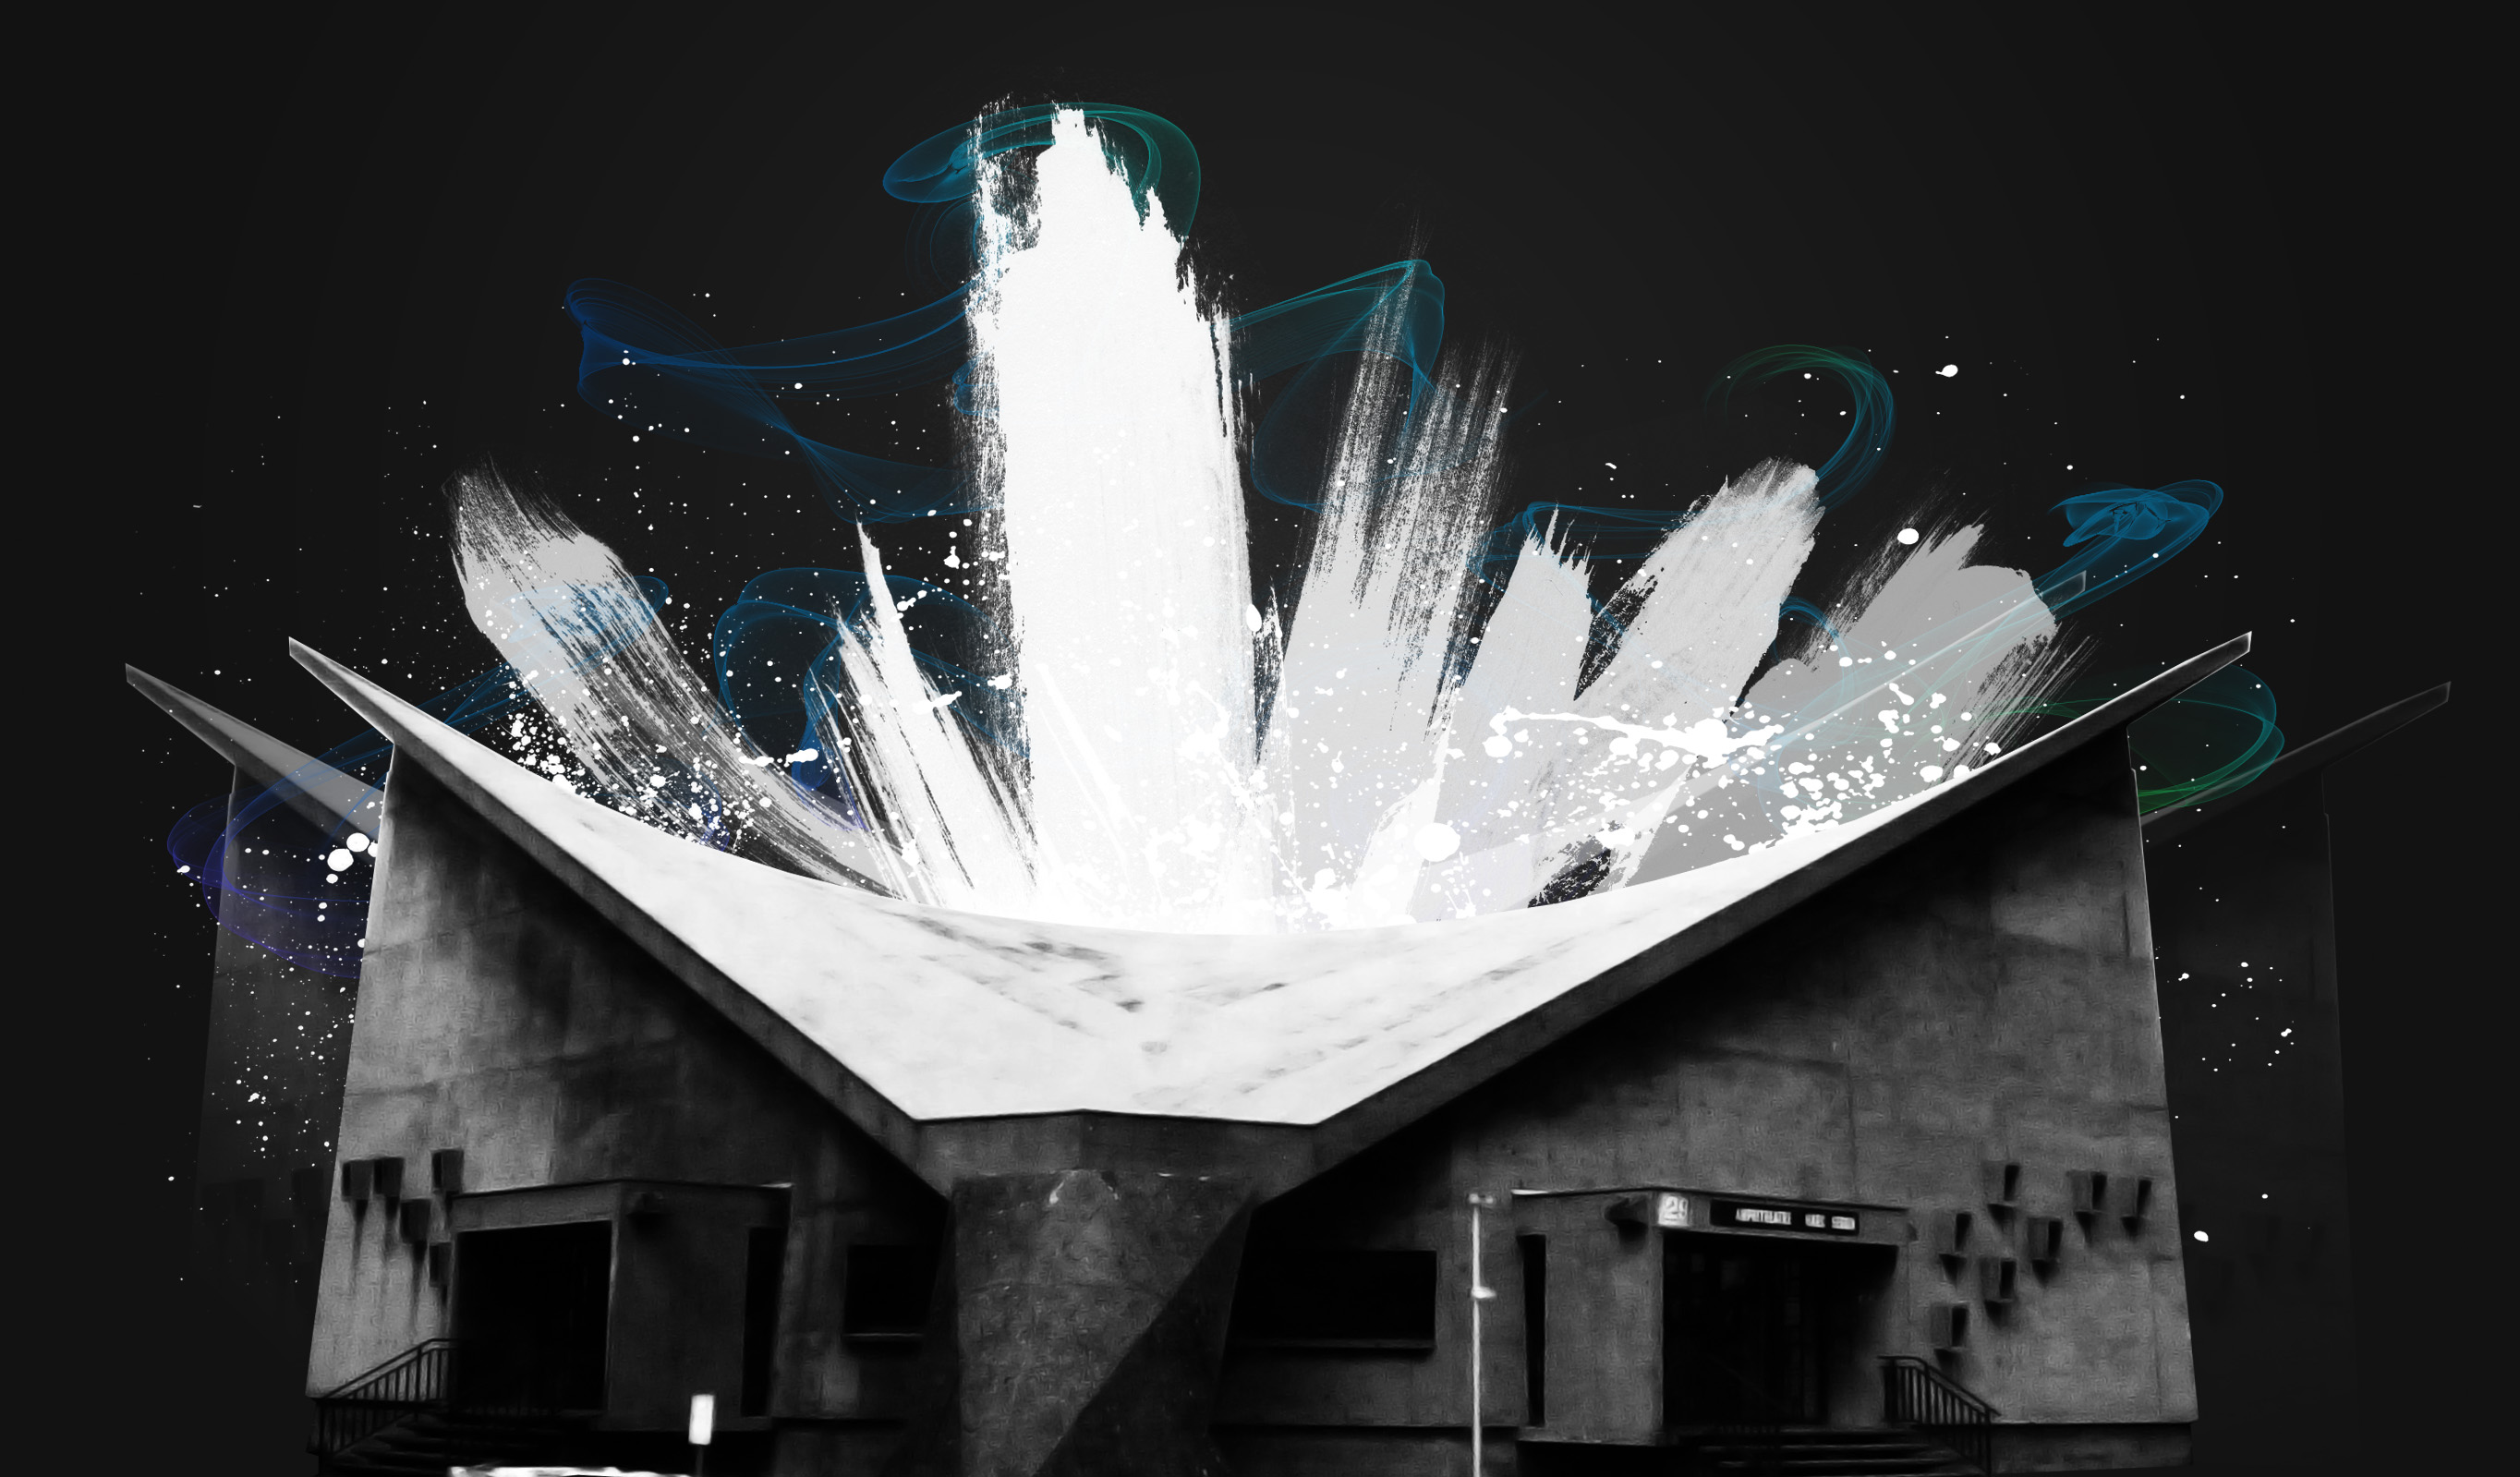
\includegraphics[width=\textwidth]{img/amphi.jpg}\\
            Première esquisse pour la bâche du BdE
        \end{center}

        \begin{center}
            %TODO inclure les autres travaux.
            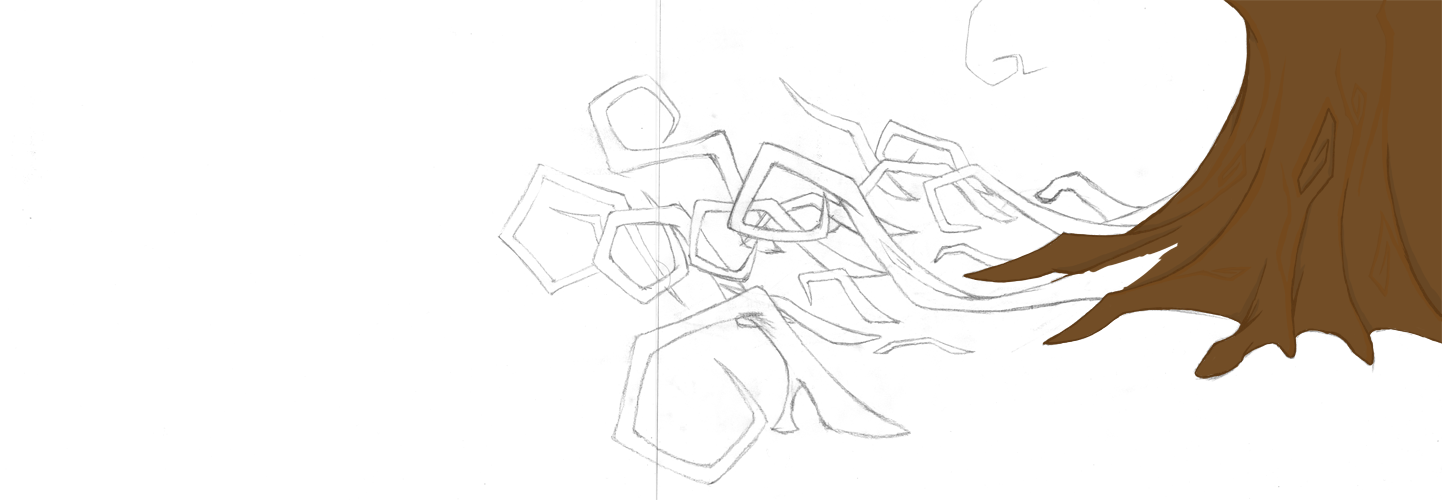
\includegraphics[width=\textwidth]{img/arbre.png}
            
\includegraphics[width=\textwidth]{img/mde.png}
            
\includegraphics[width=\textwidth]{img/mde+arbre.png}
            Différentes ébauche et évolution du travail sur la bâche du BdE.
        \end{center}
            
    \subsection{24h de l'Insa}
    
        \subsubsection{36èeme édition - 2010}
    
            \begin{center}
                \fbox{
\includegraphics[width=0.3\textwidth]{img/preAffiche.png}}
                \fbox{
\includegraphics[width=0.3\textwidth]{img/preAffiche_panda.png}}
                \fbox{
\includegraphics[width=0.3\textwidth]{img/preAffiche_panda_2.png}}\\    
                \fbox{
\includegraphics[width=0.3\textwidth]{img/preAffiche_panda_2leaf_date1.png}}
                \fbox{
\includegraphics[width=0.3\textwidth]{img/preAffiche_panda_2leaf_date2.png}}
                \fbox{
\includegraphics[width=0.3\textwidth]{img/preAffiche_panda_2hot.png}}\\
                \fbox{
\includegraphics[width=0.3\textwidth]{img/preAffiche_panda_3.png}}
                \fbox{
\includegraphics[width=0.3\textwidth]{img/preAffiche_panda_3-2.png}}
                \fbox{
\includegraphics[width=0.3\textwidth]{img/preAffiche_panda_3-3.png}}\\
                Suivi des étapes dans le travail sur l'affiche des 24h de l'insa, 36ème édition - 2010
            \end{center}
            
            \begin{center}
                \fbox{
\includegraphics[width=0.48\textwidth]{img/affiche_concert.png}}
                \fbox{
\includegraphics[width=0.48\textwidth]{img/affiche-concerts-v4-flat2.jpg}}\\
                Affiche proposé et affiche finale  
            \end{center}
            
        \subsubsection{37èeme édition - 2011}            
            
            \begin{center}        
                \fbox{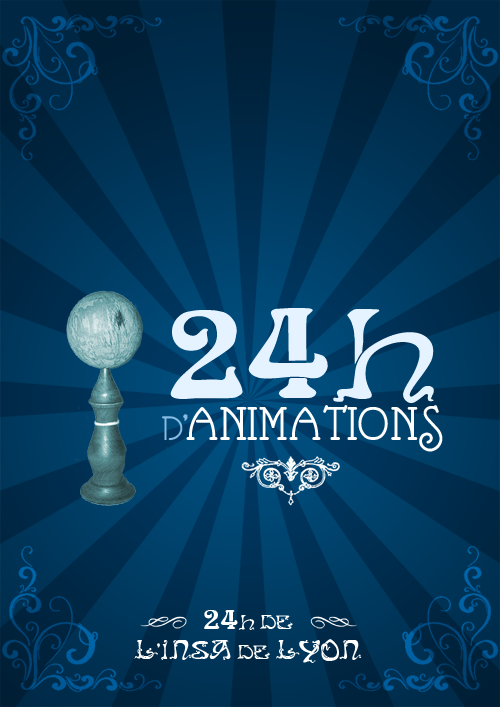
\includegraphics[width=0.3\textwidth]{img/old-preview-animations.png}}
                \fbox{
\includegraphics[width=0.3\textwidth]{img/old-preview-courses.png}}
                \fbox{
\includegraphics[width=0.3\textwidth]{img/old-preview-concert.png}}
                Présentation d'un thème de communication intitulé \emph{Old School}
            \end{center}
            
            \begin{center}           
                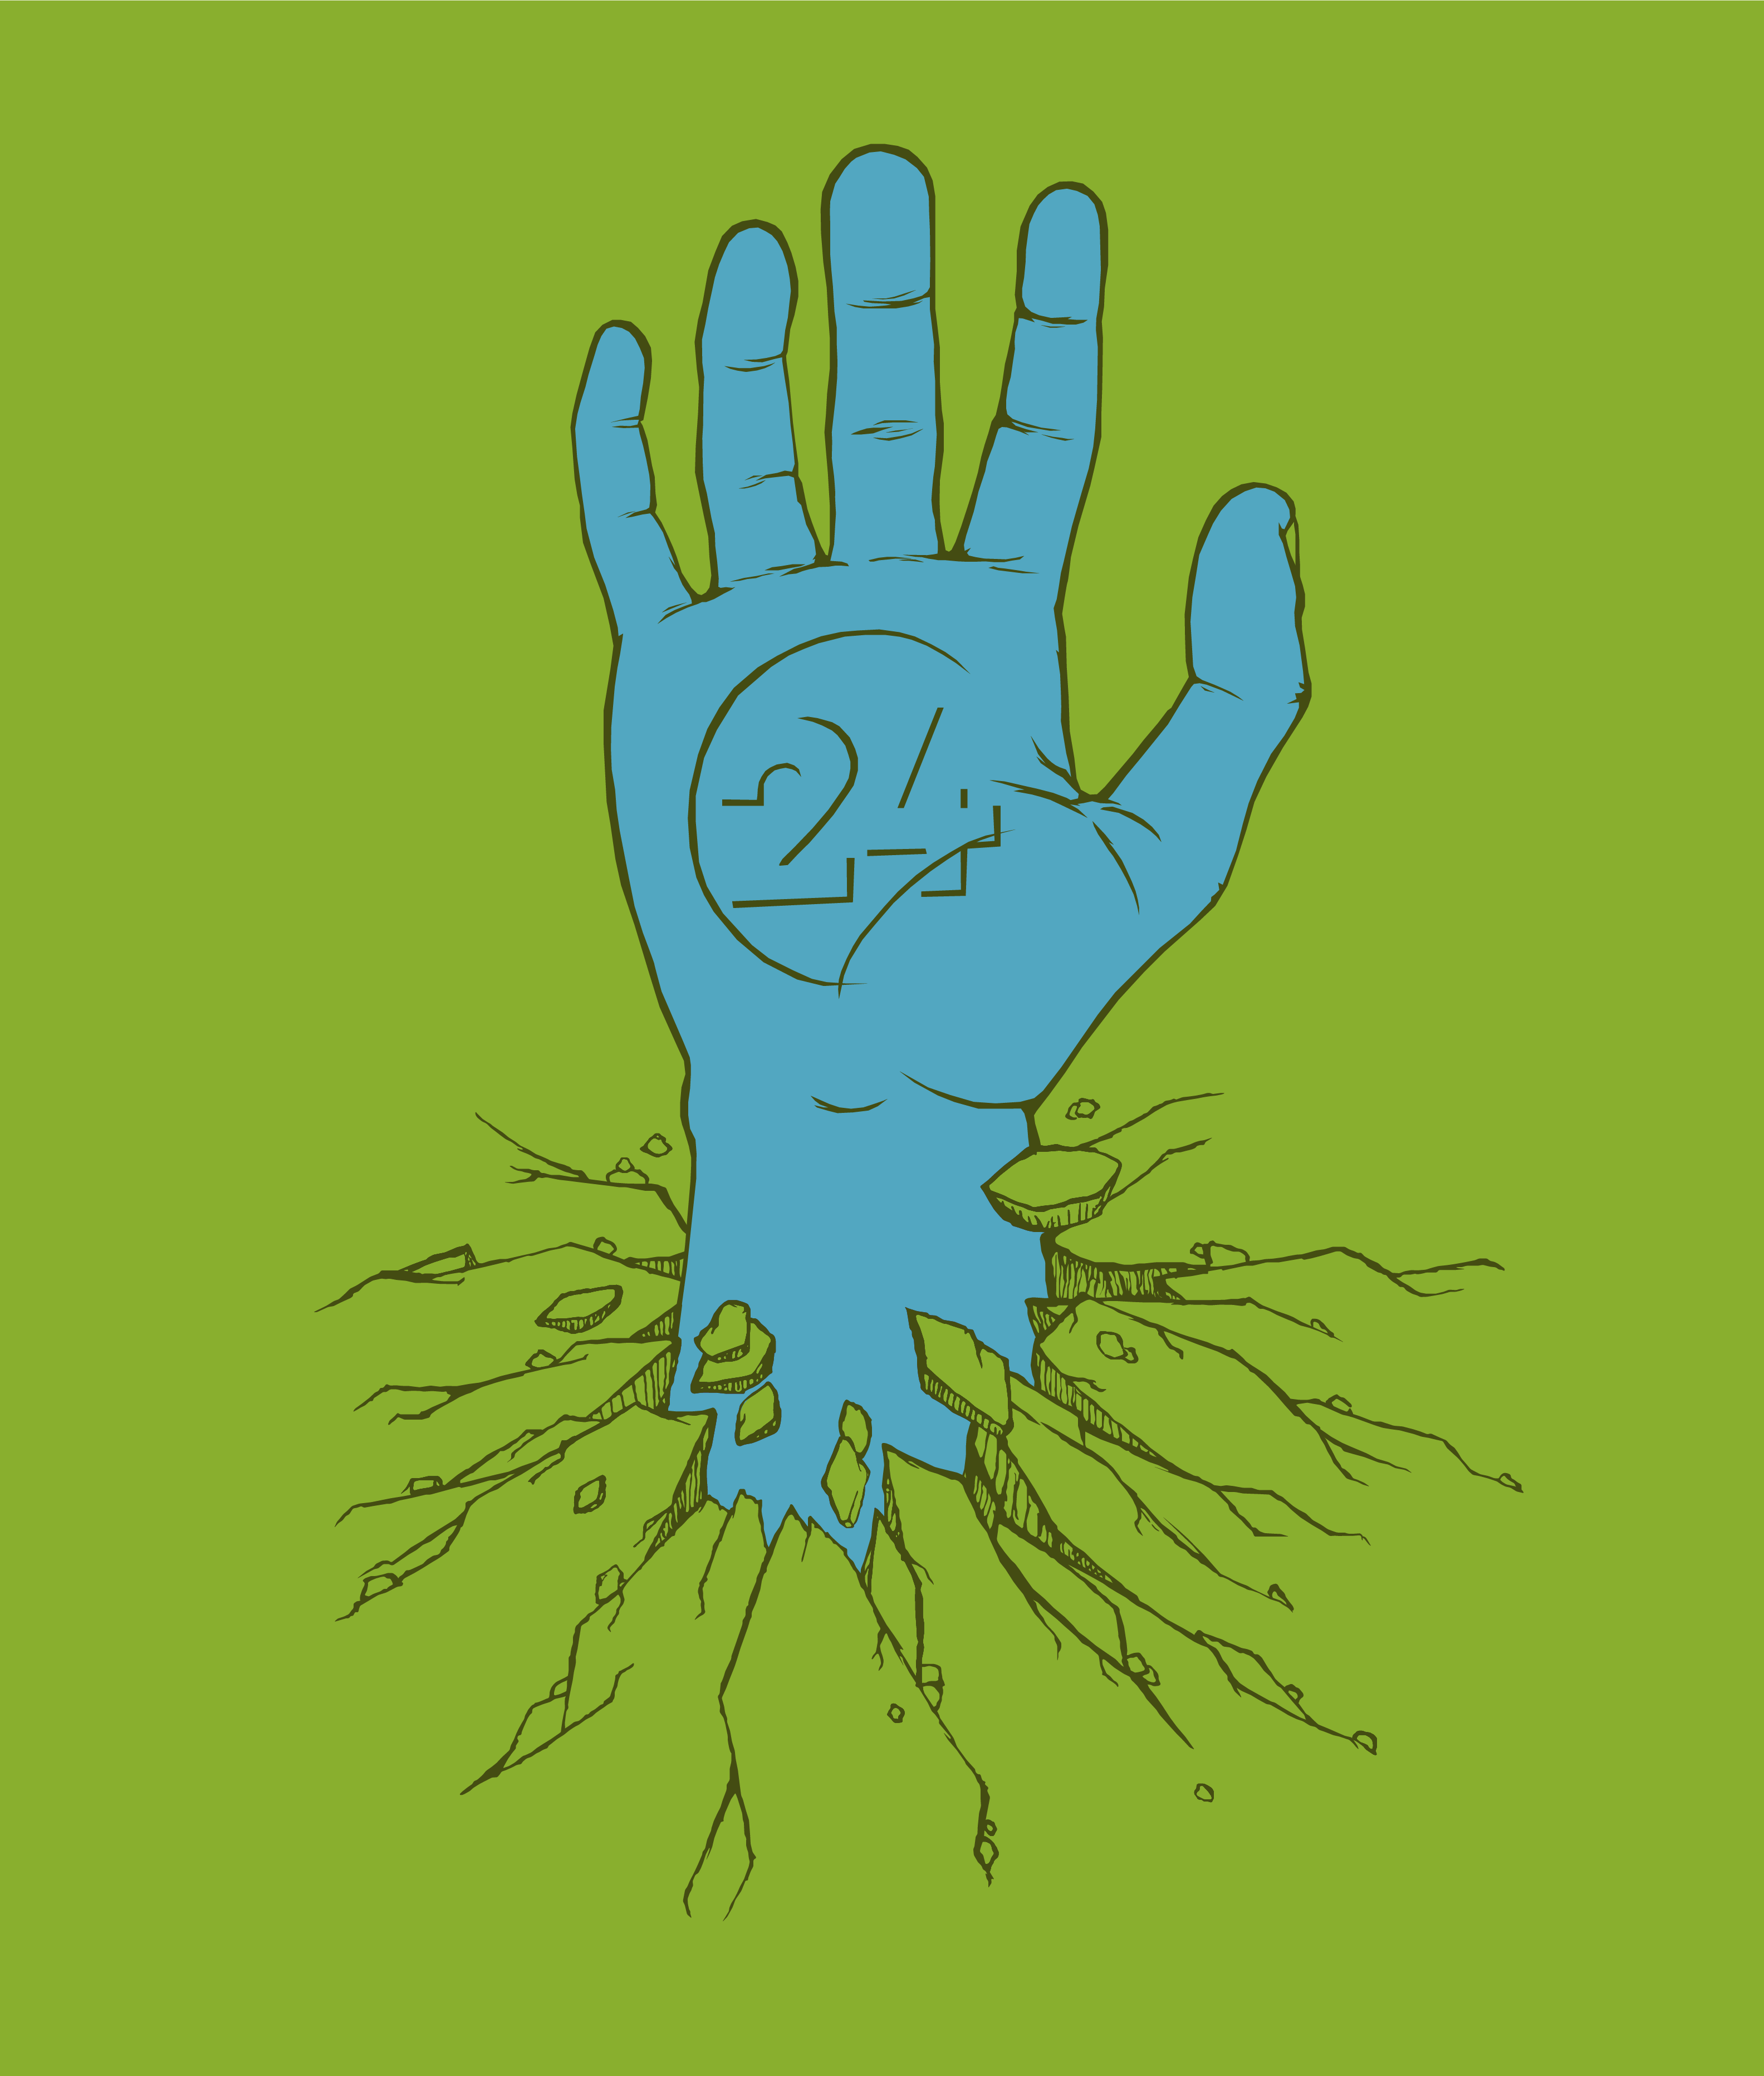
\includegraphics[width=\textwidth]{img/main.png}\\
                ~\\
                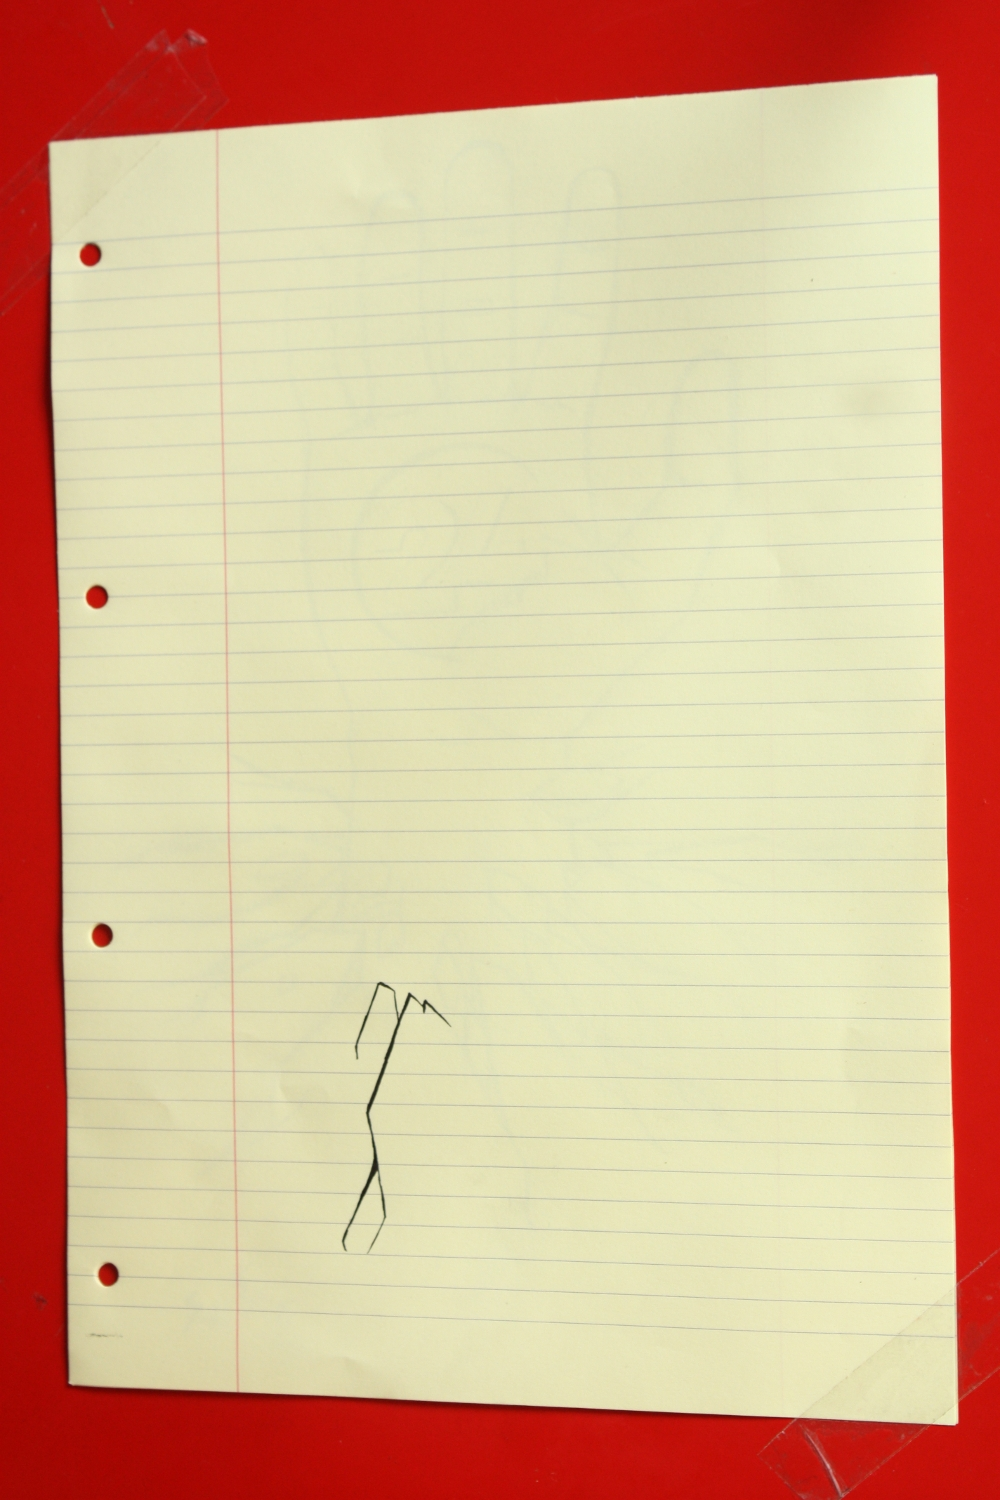
\includegraphics[width=0.24\textwidth]{img/IMG_5730.JPG}
                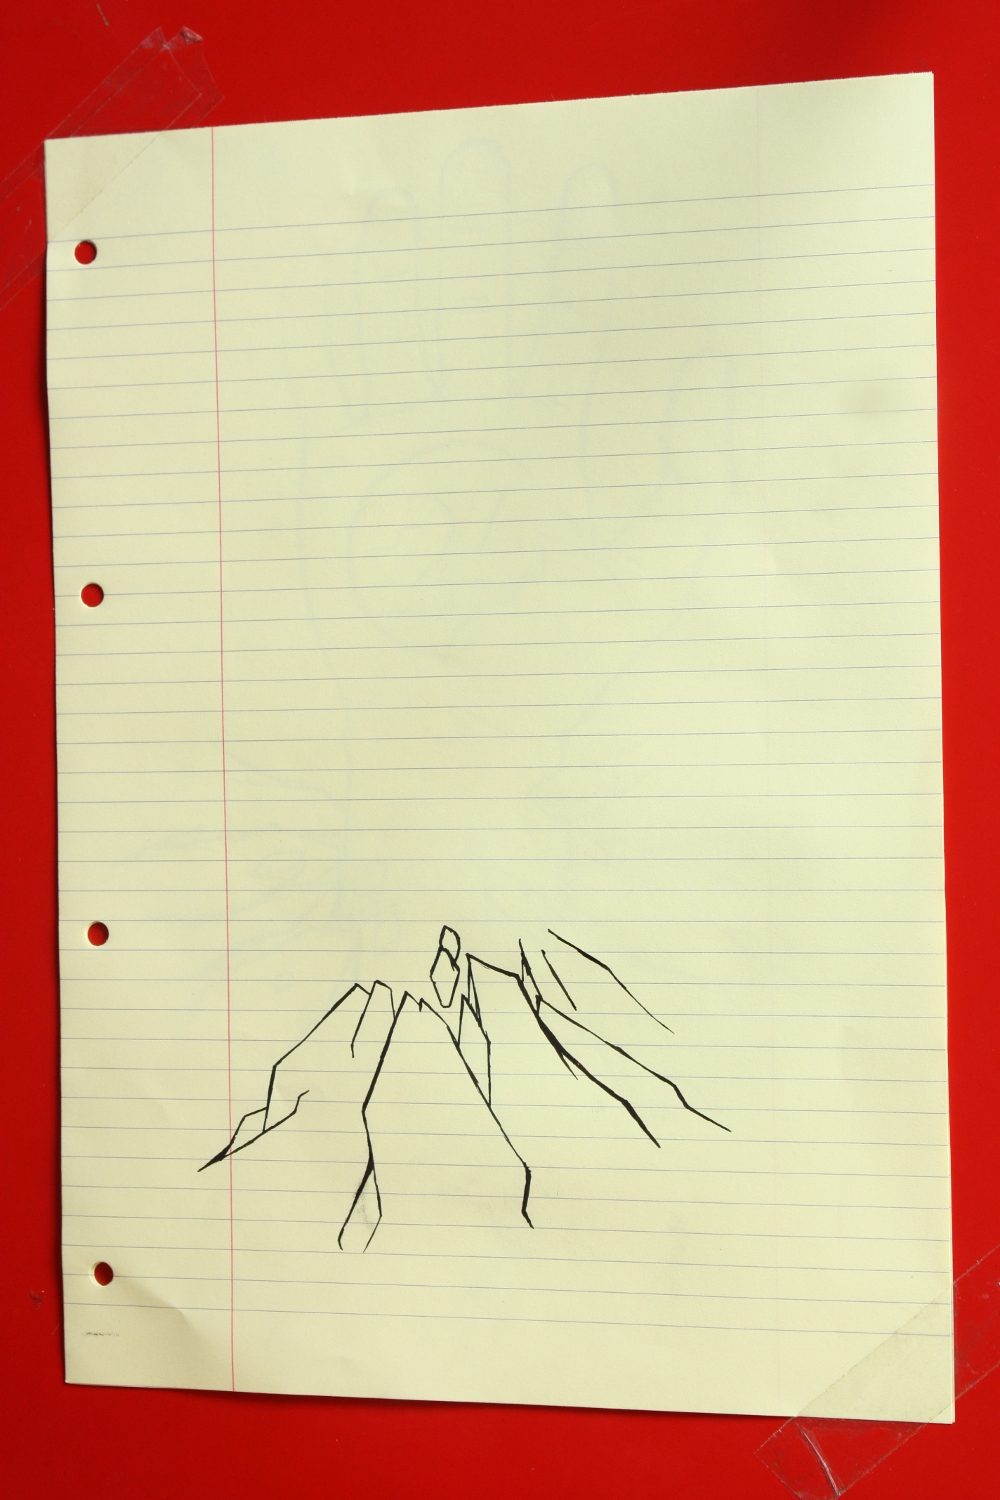
\includegraphics[width=0.24\textwidth]{img/IMG_5741.JPG}
                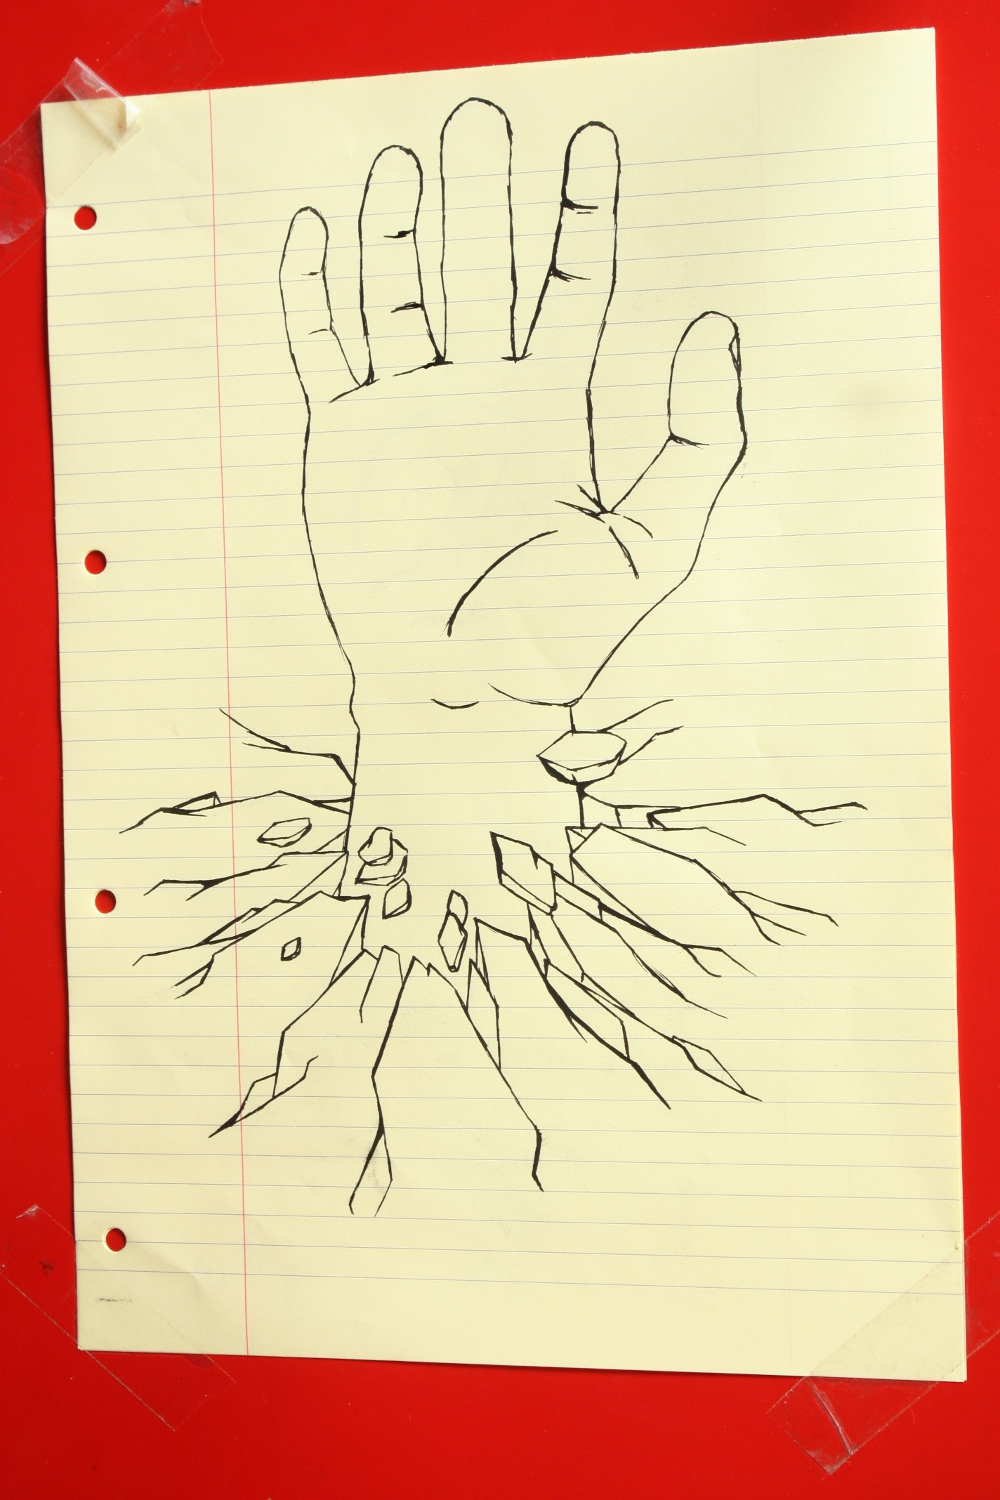
\includegraphics[width=0.24\textwidth]{img/IMG_5792.JPG}
                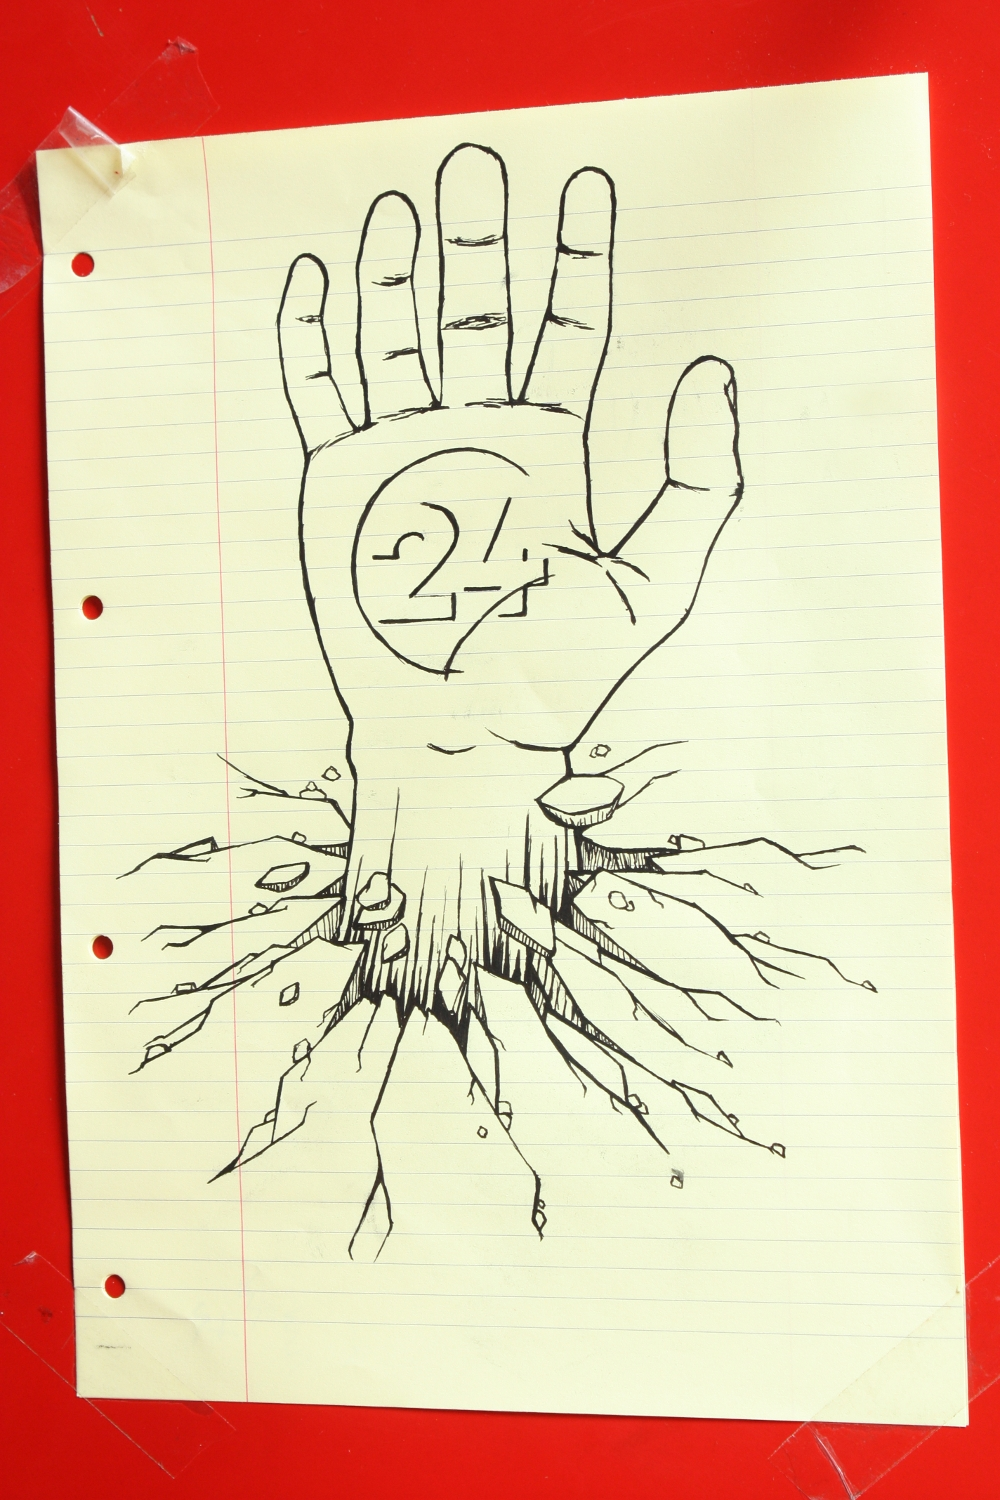
\includegraphics[width=0.24\textwidth]{img/IMG_5848.JPG}
                Une idée de visuel pour un T-Shirt vente
            \end{center}
            
            \begin{center}                     
                
\includegraphics[width=\textwidth]{img/splash24.png}
                Travail sur le logo de l'association, pour le thème \textit{tâches de peintures}
            \end{center}
                        
            \begin{center}
                
\includegraphics[width=\textwidth]{img/logo-TShirt-bichro.png}
                Proposition de visuel pour un T-Shirt vente
            \end{center}
                
            \begin{center}    
                \fbox{
\includegraphics[width=\textwidth]{img/affiche-soiree.png}}
                Proposition d'affiche concert  
            \end{center}
            
    \subsection{AEDI}
            
        \begin{center}
            %\fbox{
\includegraphics[width=0.3\textwidth]{img/WTFBBQjp.jpg}}
            \fbox{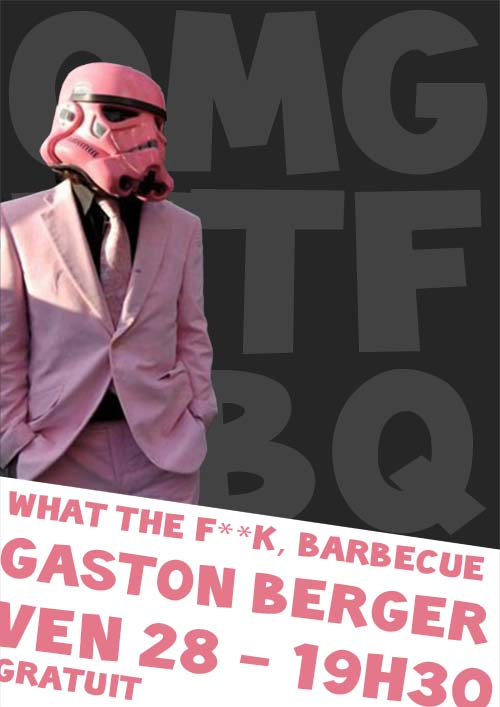
\includegraphics[width=0.3\textwidth]{img/WTFBBQstorm.jpg}}
            \fbox{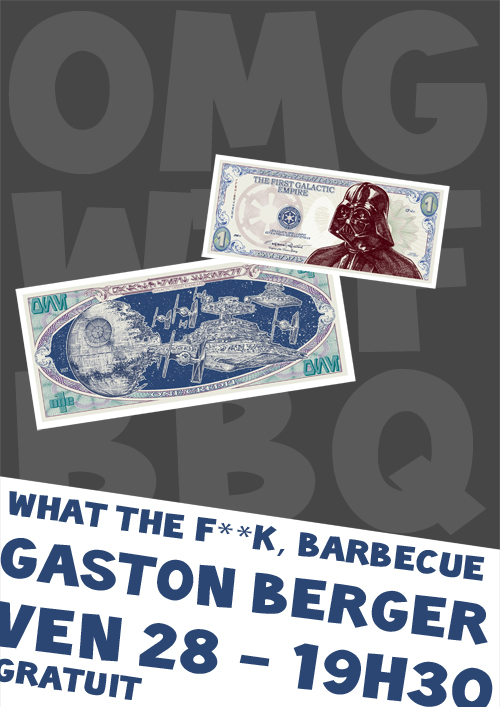
\includegraphics[width=0.3\textwidth]{img/WTFBBQsw.jpg}}
            %\fbox{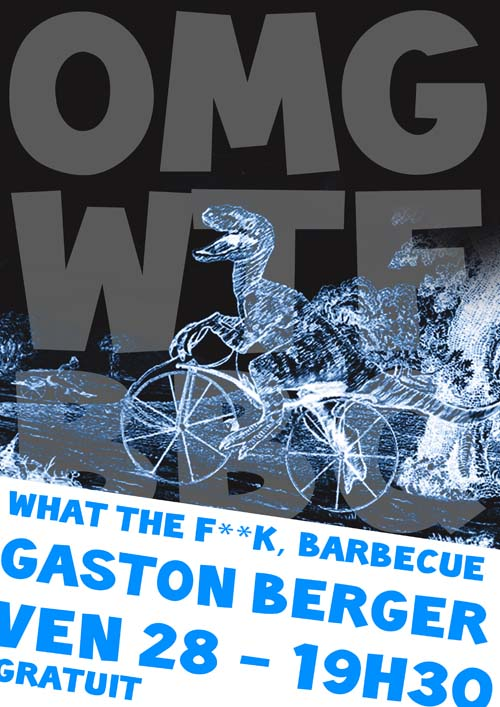
\includegraphics[width=0.3\textwidth]{img/WTFBBQvelo.jpg}}
            \fbox{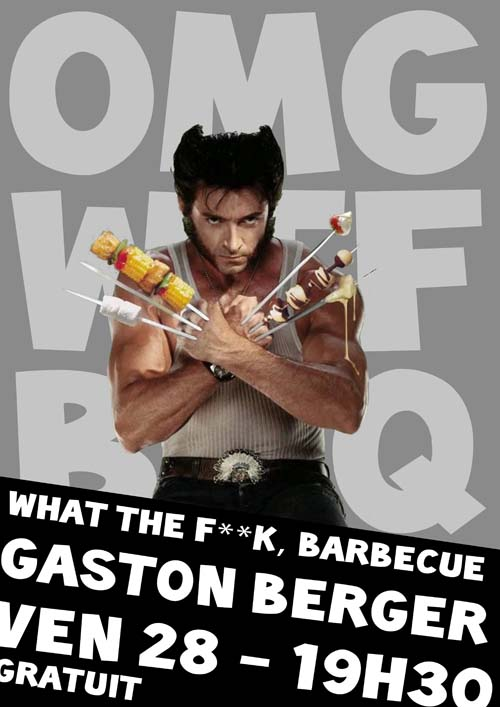
\includegraphics[width=0.3\textwidth]{img/WTFBBQwolv.jpg}}
            %\fbox{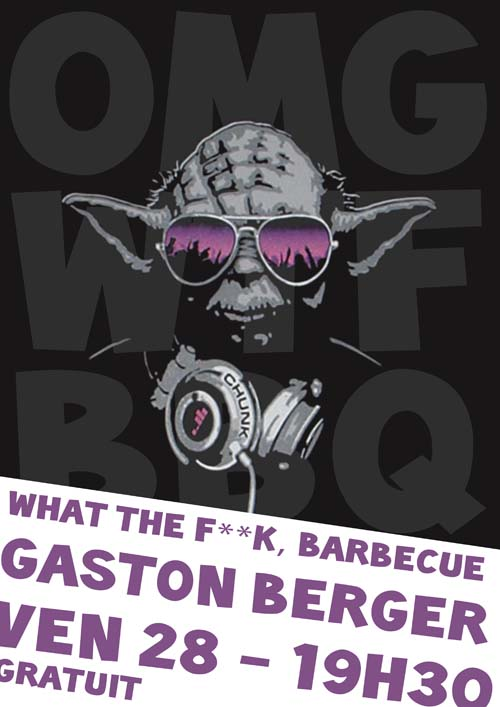
\includegraphics[width=0.3\textwidth]{img/WTFBBQyoda.jpg}}
            Affiches pour le barbecue de fin d'année de l'AEDI
        \end{center}
        
        \begin{center}
            \centering
            
\includegraphics[width=0.9\textwidth]{img/yoda-or.jpg}\\
            Visuel de T-Shirt pour la promotion 52
        \end{center}




